\begin{savequote}[8cm]
\end{savequote}

\chapter{\label{app:1-cardiophys}Appendices}

\minitoc

\section{Summary Tables}
\label{App:Summary_Tables}
All the sample simulation/reconstruction conditions tested for ND-GAr and ND-GAr-Lite are summarized in Table \ref{Tab:GAr} and \ref{Tab:Lite} respectively. All test samples are identified by a code composed of up to three numbers and a letter. The main number $n$ identifies a specific set of simulation conditions, while the other numbers and letters or lack thereof characterize the reconstruction:
\begin{itemize}
    \item $\textbf{n:}$ the seeding step is "cheated" i.e. the EKF is applied using MC true values as initial guesses
    \item $\textbf{n.5:}$ the seeding is done using the ALICE 3-point method
    \item $\textbf{n.6:}$ the seeding is done using the ILRM method
    \item $\textbf{n.x.1:}$ the energy loss correction is applied to the seeding
    \item $\textbf{n.x.2:}$ the energy loss and multiple scattering correction are both applied to the seeding
    \item $\textbf{n.x.3:}$ the multiple scattering correction is applied to the seeding
    \item $\textbf{n.x.y a:}$ the EKF is applied to a realistic seed 
    \item $\textbf{n.x.y b:}$ the EKF is applied to a realistic seed, with additional energy loss corrections
    \item $\textbf{n.x.y c:}$ the EKF is applied to a realistic seed, with additional energy loss and multiple scattering corrections
    \item $\textbf{n.x.y d:}$ the EKF is applied to a realistic seed, with additional multiple scattering corrections   
\end{itemize}
\begin{table}[!hb]
        \begin{adjustwidth}{-1.2in}{-1.2in}
    \fontsize{6}{10}\selectfont 
    \centering
    \setlength\tabcolsep{1.5pt}
    \centering
    \begin{tabular}{|l|l|l|l|l|l|l|l|l|l|l|l|l|l|l|l|l|}
    \hline
        ~ & \multicolumn{4}{|c|}{\textbf{Monte Carlo}} & \multicolumn{6}{|c|}{\textbf{Seed}}& \multicolumn{2}{|c|}{\textbf{Kalman Filter}}& \multicolumn{2}{|c|}{\textbf{Spectrum}} & \multicolumn{2}{|c|}{\textbf{Geometry}}\\ \hline
        ~ & $\sigma_{yz}$ & dE/dx & pidCode & MS & Standalone & ALICE & dE/dx Corr & MS Corr & Cheated & Realistic & dE/dx Corr & MS Corr & Fixed p & Random & densScaling & resScaling \\ \hline
        0.5 & \checkmark& ~ & 1 & ~ & \checkmark& \checkmark& ~ & ~ & ~ & ~ & ~ & ~ & \checkmark& ~ & 10 & 1 \\ \hline
        0.5a & \checkmark& ~ & 1 & ~ & ~ & \checkmark& ~ & ~ & ~ & \checkmark& ~ & ~ & \checkmark& ~ & 10 & 1 \\ \hline
        1.5 & \checkmark& \checkmark& 1 & ~ & \checkmark& \checkmark& ~ & ~ & ~ & ~ & ~ & ~ & \checkmark& ~ & 10 & 1 \\ \hline
        1.5a & \checkmark& \checkmark& 1 & ~ & ~ & \checkmark& ~ & ~ & ~ & \checkmark& ~ & ~ & \checkmark& ~ & 10 & 1 \\ \hline
        1.5b & \checkmark& \checkmark& 1 & ~ & ~ & \checkmark& ~ & ~ & ~ & \checkmark& \checkmark& ~ & \checkmark& ~ & 10 & 1 \\ \hline
        1.5.1 & \checkmark& \checkmark& 1 & ~ & \checkmark& \checkmark& ~ & ~ & ~ & ~ & ~ & ~ & \checkmark& ~ & 10 & 1 \\ \hline
        1.5.1a & \checkmark& \checkmark& 1 & ~ & ~ & \checkmark& \checkmark& ~ & ~ & \checkmark& ~ & ~ & \checkmark& ~ & 10 & 1 \\ \hline
        1.5.1b & \checkmark& \checkmark& 1 & ~ & ~ & \checkmark& \checkmark& ~ & ~ & \checkmark& \checkmark& ~ & \checkmark& ~ & 10 & 1 \\ \hline
        2.5 & \checkmark& ~ & 1 & \checkmark& \checkmark& \checkmark& ~ & ~ & ~ & ~ & ~ & ~ & \checkmark& ~ & 10 & 1 \\ \hline
        2.5a & \checkmark& ~ & 1 & \checkmark& ~ & \checkmark& ~ & ~ & ~ & \checkmark& ~ & ~ & \checkmark& ~ & 10 & 1 \\ \hline
        2.5d & \checkmark& ~ & 1 & \checkmark& ~ & \checkmark& ~ & ~ & ~ & \checkmark& ~ & \checkmark& \checkmark& ~ & 10 & 1 \\ \hline
        2.5.3 & \checkmark& ~ & 1 & \checkmark& \checkmark& \checkmark& ~ & \checkmark& ~ & ~ & ~ & ~ & \checkmark& ~ & 10 & 1 \\ \hline
        2.5.3a & \checkmark& ~ & 1 & \checkmark& ~ & \checkmark& ~ & \checkmark& ~ & \checkmark& ~ & ~ & \checkmark& ~ & 10 & 1 \\ \hline
        2.5.3d & \checkmark& ~ & 1 & \checkmark& ~ & \checkmark& ~ & \checkmark& ~ & \checkmark& ~ & \checkmark& \checkmark& ~ & 10 & 1 \\ \hline
        3.5 & \checkmark& \checkmark& 1 & \checkmark& \checkmark& \checkmark& ~ & ~ & ~ & ~ & ~ & ~ & \checkmark& ~ & 10 & 1 \\ \hline
        3.5a & \checkmark& \checkmark& 1 & \checkmark& ~ & \checkmark& ~ & ~ & ~ & \checkmark& ~ & ~ & \checkmark& ~ & 10 & 1 \\ \hline
        3.5b & \checkmark& \checkmark& 1 & \checkmark& ~ & \checkmark& ~ & ~ & ~ & \checkmark& \checkmark& ~ & \checkmark& ~ & 10 & 1 \\ \hline
        3.5c & \checkmark& \checkmark& 1 & \checkmark& ~ & \checkmark& ~ & ~ & ~ & \checkmark& \checkmark& \checkmark& \checkmark& ~ & 10 & 1 \\ \hline
        3.5d & \checkmark& \checkmark& 1 & \checkmark& ~ & \checkmark& ~ & ~ & ~ & \checkmark& ~ & \checkmark& \checkmark& ~ & 10 & 1 \\ \hline
        3.5 & \checkmark& \checkmark& 1 & \checkmark& \checkmark& \checkmark& \checkmark& ~ & ~ & ~ & ~ & ~ & \checkmark& ~ & 10 & 1 \\ \hline
        3.5a & \checkmark& \checkmark& 1 & \checkmark& ~ & \checkmark& \checkmark& ~ & ~ & \checkmark& ~ & ~ & \checkmark& ~ & 10 & 1 \\ \hline
        3.5b & \checkmark& \checkmark& 1 & \checkmark& ~ & \checkmark& \checkmark& ~ & ~ & \checkmark& \checkmark& ~ & \checkmark& ~ & 10 & 1 \\ \hline
        3.5c & \checkmark& \checkmark& 1 & \checkmark& ~ & \checkmark& \checkmark& ~ & ~ & \checkmark& \checkmark& \checkmark& \checkmark& ~ & 10 & 1 \\ \hline
        3.5d & \checkmark& \checkmark& 1 & \checkmark& ~ & \checkmark& \checkmark& ~ & ~ & \checkmark& ~ & \checkmark& \checkmark& ~ & 10 & 1 \\ \hline
        3.5.2 & \checkmark& \checkmark& 1 & \checkmark& \checkmark& \checkmark& \checkmark& \checkmark& ~ & ~ & ~ & ~ & \checkmark& ~ & 10 & 1 \\ \hline
        3.5.2a & \checkmark& \checkmark& 1 & \checkmark& ~ & \checkmark& \checkmark& \checkmark& ~ & \checkmark& ~ & ~ & \checkmark& ~ & 10 & 1 \\ \hline
        3.5.2b & \checkmark& \checkmark& 1 & \checkmark& ~ & \checkmark& \checkmark& \checkmark& ~ & \checkmark& \checkmark& ~ & \checkmark& ~ & 10 & 1 \\ \hline
        3.5.2c & \checkmark& \checkmark& 1 & \checkmark& ~ & \checkmark& \checkmark& \checkmark& ~ & \checkmark& \checkmark& \checkmark& \checkmark& ~ & 10 & 1 \\ \hline
        3.5.2d & \checkmark& \checkmark& 1 & \checkmark& ~ & \checkmark& \checkmark& \checkmark& ~ & \checkmark& ~ & \checkmark& \checkmark& ~ & 10 & 1 \\ \hline
        4.5.2c & \checkmark& \checkmark& 1 & \checkmark& ~ & \checkmark& \checkmark& \checkmark& ~ & \checkmark& \checkmark& \checkmark& ~ & \checkmark& 10 & 1 \\ \hline
        5.5.2c & \checkmark& \checkmark& [0,4] & \checkmark& ~ & \checkmark& \checkmark& \checkmark& ~ & \checkmark& \checkmark& \checkmark& ~ & \checkmark& [0.01,10] & [0.01,2] \\ \hline
    \end{tabular}
    \end{adjustwidth} 
    \caption{Summary of all sample conditions used for ND-GAr EKF tests}
    \label{Tab:GAr}
\end{table}


\begin{table}[!ht]
    \begin{adjustwidth}{-1.2in}{-1.2in}
    \fontsize{5}{8}\selectfont 
    \centering
    \setlength\tabcolsep{1.5pt}
    \begin{tabular}{|l|l|l|l|l|l|l|l|l|l|l|l|l|l|l|l|l|l|l|l|}
    \hline
        ~ & \multicolumn{6}{|c|}{\textbf{Monte Carlo}}  & \multicolumn{7}{|c|}{\textbf{Seed}} & \multicolumn{2}{|c|}{\textbf{Kalman Filter}} & \multicolumn{2}{|c|}{\textbf{Spectrum}} & \multicolumn{2}{|c|}{\textbf{Geometry}}  \\ \hline
        ~ & $\sigma_{yz}$ & dE/dx & Gauss $\sigma_E$ & Landau $\sigma_E$ & MS & Garsoft& Alone & ALICE & ILRM & dE/dx & MS & Cheated & Realistic& dE/dx Corr & MS Corr & Fixed p & Random & 5 planes & 6 planes \\ \hline
        0 & ~ & ~ & ~ & ~ & ~ & ~ & ~ & ~ & ~ & ~ & ~ & \checkmark & ~ & ~ & ~ & ~ & \checkmark & \checkmark & ~ \\ \hline
        0.5 & ~ & ~ & ~ & ~ & ~ & ~ & \checkmark & \checkmark & ~ & ~ & ~ & ~ & ~ & ~ & ~ & ~ & \checkmark & \checkmark & ~ \\ \hline
        0.5a & ~ & ~ & ~ & ~ & ~ & ~ & ~ & \checkmark & ~ & ~ & ~ & ~ & \checkmark & ~ & ~ & ~ & \checkmark & \checkmark & ~ \\ \hline
        1 & \checkmark & ~ & ~ & ~ & ~ & ~ & ~ & ~ & ~ & ~ & ~ & \checkmark & ~ & ~ & ~ & ~ & \checkmark & \checkmark & ~ \\ \hline
        1.5 & \checkmark & ~ & ~ & ~ & ~ & ~ & \checkmark & \checkmark & ~ & ~ & ~ & ~ & ~ & ~ & ~ & ~ & \checkmark & \checkmark & ~ \\ \hline
        1.5a & \checkmark & ~ & ~ & ~ & ~ & ~ & ~ & \checkmark & ~ & ~ & ~ & ~ & \checkmark & ~ & ~ & ~ & \checkmark & \checkmark & ~ \\ \hline
        2 & ~ & \checkmark & ~ & ~ & ~ & ~ & ~ & ~ & ~ & ~ & ~ & \checkmark & ~ & ~ & ~ & ~ & \checkmark & \checkmark & ~ \\ \hline
        2b & ~ & \checkmark & ~ & ~ & ~ & ~ & ~ & ~ & ~ & ~ & ~ & \checkmark & ~ & \checkmark & ~ & ~ & \checkmark & \checkmark & ~ \\ \hline
        2.5 & ~ & \checkmark & ~ & ~ & ~ & ~ & \checkmark & \checkmark & ~ & ~ & ~ & ~ & ~ & ~ & ~ & ~ & \checkmark & \checkmark & ~ \\ \hline
        2.5a & ~ & \checkmark & ~ & ~ & ~ & ~ & ~ & \checkmark & ~ & ~ & ~ & ~ & \checkmark & ~ & ~ & ~ & \checkmark & \checkmark & ~ \\ \hline
        2.5b & ~ & \checkmark & ~ & ~ & ~ & ~ & ~ & \checkmark & ~ & ~ & ~ & ~ & \checkmark & \checkmark & ~ & ~ & \checkmark & \checkmark & ~ \\ \hline
        3 & ~ & \checkmark & \checkmark & ~ & ~ & ~ & ~ & \checkmark & ~ & ~ & ~ & \checkmark & ~ & ~ & ~ & ~ & \checkmark & \checkmark & ~ \\ \hline
        3b & ~ & \checkmark & \checkmark & ~ & ~ & ~ & ~ & \checkmark & ~ & ~ & ~ & \checkmark & ~ & \checkmark & ~ & ~ & \checkmark & \checkmark & ~ \\ \hline
        3.5 & ~ & \checkmark & \checkmark & ~ & ~ & ~ & \checkmark & \checkmark & ~ & ~ & ~ & ~ & ~ & ~ & ~ & ~ & \checkmark & \checkmark & ~ \\ \hline
        3.5a & ~ & \checkmark & \checkmark & ~ & ~ & ~ & ~ & \checkmark & ~ & ~ & ~ & ~ & \checkmark & ~ & ~ & ~ & \checkmark & \checkmark & ~ \\ \hline
        3.5b & ~ & \checkmark & \checkmark & ~ & ~ & ~ & ~ & \checkmark & ~ & ~ & ~ & ~ & \checkmark & \checkmark & ~ & ~ & \checkmark & \checkmark & ~ \\ \hline
        4 & ~ & \checkmark & ~ & \checkmark & ~ & ~ & ~ & \checkmark & ~ & ~ & ~ & \checkmark & ~ & ~ & ~ & ~ & \checkmark & \checkmark & ~ \\ \hline
        4b & ~ & \checkmark & ~ & \checkmark & ~ & ~ & ~ & \checkmark & ~ & ~ & ~ & \checkmark & ~ & \checkmark & ~ & ~ & \checkmark & \checkmark & ~ \\ \hline
        4.5 & ~ & \checkmark & ~ & \checkmark & ~ & ~ & \checkmark & \checkmark & ~ & ~ & ~ & ~ & ~ & ~ & ~ & ~ & \checkmark & \checkmark & ~ \\ \hline
        4.5a & ~ & \checkmark & ~ & \checkmark & ~ & ~ & ~ & \checkmark & ~ & ~ & ~ & ~ & \checkmark & ~ & ~ & ~ & \checkmark & \checkmark & ~ \\ \hline
        4.5b & ~ & \checkmark & ~ & \checkmark & ~ & ~ & ~ & \checkmark & ~ & ~ & ~ & ~ & \checkmark & \checkmark & ~ & ~ & \checkmark & \checkmark & ~ \\ \hline
        5.5 & ~ & \checkmark & ~ & ~ & ~ & ~ & \checkmark & \checkmark & ~ & ~ & ~ & ~ & ~ & ~ & ~ & \checkmark & ~ & \checkmark & ~ \\ \hline
        5.5a & ~ & \checkmark & ~ & ~ & ~ & ~ & ~ & \checkmark & ~ & ~ & ~ & ~ & \checkmark & ~ & ~ & \checkmark & ~ & \checkmark & ~ \\ \hline
        5.5b & ~ & \checkmark & ~ & ~ & ~ & ~ & ~ & \checkmark & ~ & ~ & ~ & ~ & \checkmark & \checkmark & ~ & \checkmark & ~ & \checkmark & ~ \\ \hline
        6.5 & ~ & \checkmark & ~ & ~ & ~ & ~ & \checkmark & \checkmark & ~ & ~ & ~ & ~ & ~ & ~ & ~ & \checkmark & ~ & ~ & \checkmark \\ \hline
        6.5a & ~ & \checkmark & ~ & ~ & ~ & ~ & ~ & \checkmark & ~ & ~ & ~ & ~ & \checkmark & ~ & ~ & \checkmark & ~ & ~ & \checkmark \\ \hline
        6.5b & ~ & \checkmark & ~ & ~ & ~ & ~ & ~ & \checkmark & ~ & ~ & ~ & ~ & \checkmark & \checkmark & ~ & \checkmark & ~ & ~ & \checkmark \\ \hline
        7.5 & ~ & \checkmark & \checkmark & ~ & ~ & ~ & \checkmark & \checkmark & ~ & ~ & ~ & ~ & ~ & ~ & ~ & \checkmark & ~ & ~ & \checkmark \\ \hline
        7.5a & ~ & \checkmark & \checkmark & ~ & ~ & ~ & ~ & \checkmark & ~ & ~ & ~ & ~ & \checkmark & ~ & ~ & \checkmark & ~ & ~ & \checkmark \\ \hline
        7.5b & ~ & \checkmark & \checkmark & ~ & ~ & ~ & ~ & \checkmark & ~ & ~ & ~ & ~ & \checkmark & \checkmark & ~ & \checkmark & ~ & ~ & \checkmark \\ \hline
        8.5 & ~ & \checkmark & ~ & \checkmark & ~ & ~ & \checkmark & \checkmark & ~ & ~ & ~ & ~ & ~ & ~ & ~ & \checkmark & ~ & ~ & \checkmark \\ \hline
        8.5a & ~ & \checkmark & ~ & \checkmark & ~ & ~ & ~ & \checkmark & ~ & ~ & ~ & ~ & \checkmark & ~ & ~ & \checkmark & ~ & ~ & \checkmark \\ \hline
        8.5b & ~ & \checkmark & ~ & \checkmark & ~ & ~ & ~ & \checkmark & ~ & ~ & ~ & ~ & \checkmark & \checkmark & ~ & \checkmark & ~ & ~ & \checkmark \\ \hline
        9.5 & \checkmark & \checkmark & \checkmark & ~ & ~ & ~ & \checkmark & \checkmark & ~ & ~ & ~ & ~ & ~ & ~ & ~ & \checkmark & ~ & ~ & \checkmark \\ \hline
        9.5a & \checkmark & \checkmark & \checkmark & ~ & ~ & ~ & ~ & \checkmark & ~ & ~ & ~ & ~ & \checkmark & ~ & ~ & \checkmark & ~ & ~ & \checkmark \\ \hline
        9.5b & \checkmark & \checkmark & \checkmark & ~ & ~ & ~ & ~ & \checkmark & ~ & ~ & ~ & ~ & \checkmark & \checkmark & ~ & \checkmark & ~ & ~ & \checkmark \\ \hline
        10.5 & \checkmark & \checkmark & ~ & \checkmark & ~ & ~ & \checkmark & \checkmark & ~ & ~ & ~ & ~ & ~ & ~ & ~ & \checkmark & ~ & ~ & \checkmark \\ \hline
        10.5a & \checkmark & \checkmark & ~ & \checkmark & ~ & ~ & ~ & \checkmark & ~ & ~ & ~ & ~ & \checkmark & ~ & ~ & \checkmark & ~ & ~ & \checkmark \\ \hline
        10.5b & \checkmark & \checkmark & ~ & \checkmark & ~ & ~ & ~ & \checkmark & ~ & ~ & ~ & ~ & \checkmark & \checkmark & ~ & \checkmark & ~ & ~ & \checkmark \\ \hline
        11.5 & ~ & \checkmark & ~ & ~ & \checkmark & ~ & \checkmark & \checkmark & ~ & ~ & ~ & ~ & ~ & ~ & ~ & \checkmark & ~ & ~ & \checkmark \\ \hline
        11.5a & ~ & \checkmark & ~ & ~ & \checkmark & ~ & ~ & \checkmark & ~ & ~ & ~ & ~ & \checkmark & ~ & ~ & \checkmark & ~ & ~ & \checkmark \\ \hline
        11.5b & ~ & \checkmark & ~ & ~ & \checkmark & ~ & ~ & \checkmark & ~ & ~ & ~ & ~ & \checkmark & \checkmark & ~ & \checkmark & ~ & ~ & \checkmark \\ \hline
        11.5c & ~ & \checkmark & ~ & ~ & \checkmark & ~ & ~ & \checkmark & ~ & ~ & ~ & ~ & \checkmark & \checkmark & \checkmark & \checkmark & ~ & ~ & \checkmark \\ \hline
        12.5 & \checkmark & \checkmark & ~ & ~ & \checkmark & ~ & \checkmark & \checkmark & ~ & ~ & ~ & ~ & ~ & ~ & ~ & \checkmark & ~ & ~ & \checkmark \\ \hline
        12.5a & \checkmark & \checkmark & ~ & ~ & \checkmark & ~ & ~ & \checkmark & ~ & ~ & ~ & ~ & \checkmark & ~ & ~ & \checkmark & ~ & ~ & \checkmark \\ \hline
        12.5b & \checkmark & \checkmark & ~ & ~ & \checkmark & ~ & ~ & \checkmark & ~ & ~ & ~ & ~ & \checkmark & \checkmark & ~ & \checkmark & ~ & ~ & \checkmark \\ \hline
        12.5c & \checkmark & \checkmark & ~ & ~ & \checkmark & ~ & ~ & \checkmark & ~ & ~ & ~ & ~ & \checkmark & \checkmark & \checkmark & \checkmark & ~ & ~ & \checkmark \\ \hline
        13.5 & \checkmark & \checkmark & \checkmark & ~ & \checkmark & ~ & \checkmark & \checkmark & ~ & ~ & ~ & ~ & ~ & ~ & ~ & \checkmark & ~ & ~ & \checkmark \\ \hline
        13.5a & \checkmark & \checkmark & \checkmark & ~ & \checkmark & ~ & ~ & \checkmark & ~ & ~ & ~ & ~ & \checkmark & ~ & ~ & \checkmark & ~ & ~ & \checkmark \\ \hline
        13.5b & \checkmark & \checkmark & \checkmark & ~ & \checkmark & ~ & ~ & \checkmark & ~ & ~ & ~ & ~ & \checkmark & \checkmark & ~ & \checkmark & ~ & ~ & \checkmark \\ \hline
        13.5c & \checkmark & \checkmark & \checkmark & ~ & \checkmark & ~ & ~ & \checkmark & ~ & ~ & ~ & ~ & \checkmark & \checkmark & \checkmark & \checkmark & ~ & ~ & \checkmark \\ \hline
        14.5 & \checkmark & \checkmark & ~ & \checkmark & \checkmark & ~ & \checkmark & \checkmark & ~ & ~ & ~ & ~ & ~ & ~ & ~ & \checkmark & ~ & ~ & \checkmark \\ \hline
        14.5a & \checkmark & \checkmark & ~ & \checkmark & \checkmark & ~ & ~ & \checkmark & ~ & ~ & ~ & ~ & \checkmark & ~ & ~ & \checkmark & ~ & ~ & \checkmark \\ \hline
        14.5b & \checkmark & \checkmark & ~ & \checkmark & \checkmark & ~ & ~ & \checkmark & ~ & ~ & ~ & ~ & \checkmark & \checkmark & ~ & \checkmark & ~ & ~ & \checkmark \\ \hline
        14.5c & \checkmark & \checkmark & ~ & \checkmark & \checkmark & ~ & ~ & \checkmark & ~ & ~ & ~ & ~ & \checkmark & \checkmark & \checkmark & \checkmark & ~ & ~ & \checkmark \\ \hline
        15.5 & ~ & ~ & ~ & ~ & ~ & \checkmark & \checkmark & \checkmark & ~ & ~ & ~ & ~ & ~ & ~ & ~ & \checkmark & ~ & ~ & \checkmark \\ \hline
        15.5a & ~ & ~ & ~ & ~ & ~ & \checkmark & ~ & \checkmark & ~ & ~ & ~ & ~ & \checkmark & ~ & ~ & \checkmark & ~ & ~ & \checkmark \\ \hline
        15.5b & ~ & ~ & ~ & ~ & ~ & \checkmark & ~ & \checkmark & ~ & ~ & ~ & ~ & \checkmark & \checkmark & ~ & \checkmark & ~ & ~ & \checkmark \\ \hline
        15.5c & ~ & ~ & ~ & ~ & ~ & \checkmark & ~ & \checkmark & ~ & ~ & ~ & ~ & \checkmark & \checkmark & \checkmark & \checkmark & ~ & ~ & \checkmark \\ \hline
        15.5.1 & ~ & ~ & ~ & ~ & ~ & \checkmark  & \checkmark & \checkmark & ~ & \checkmark & ~ & ~ & ~ & ~ & ~ & \checkmark & ~ & ~ & \checkmark \\ \hline
        15.5.1a & ~ & ~ & ~ & ~ & ~ & \checkmark  & ~ & \checkmark & ~ & \checkmark & ~ & ~ & \checkmark & ~ & ~ & \checkmark & ~ & ~ & \checkmark \\ \hline
        15.5.1b & ~ & ~ & ~ & ~ & ~ & \checkmark  & ~ & \checkmark & ~ & \checkmark & ~ & ~ & \checkmark & \checkmark & ~ & \checkmark & ~ & ~ & \checkmark \\ \hline
        15.5.1c & ~ & ~ & ~ & ~ & ~ & \checkmark & ~ & \checkmark & ~ & \checkmark & ~ & ~ & \checkmark & \checkmark & \checkmark & \checkmark & ~ & ~ & \checkmark \\ \hline
        15.5.2 & ~ & ~ & ~ & ~ & ~ & \checkmark & \checkmark & \checkmark & ~ & \checkmark & \checkmark & ~ & ~ & ~ & ~ & \checkmark & ~ & ~ & \checkmark \\ \hline
        15.5.2a & ~ & ~ & ~ & ~ & ~ & \checkmark & ~ & \checkmark & ~ & \checkmark & \checkmark & ~ & \checkmark & ~ & ~ & \checkmark & ~ & ~ & \checkmark \\ \hline
        15.5.2b & ~ & ~ & ~ & ~ & ~ & \checkmark & ~ & \checkmark & ~ & \checkmark & \checkmark & ~ & \checkmark & \checkmark & ~ & \checkmark & ~ & ~ & \checkmark \\ \hline
        15.5.2c & ~ & ~ & ~ & ~ & ~ & \checkmark & ~ & \checkmark & ~ & \checkmark & \checkmark & ~ & \checkmark & \checkmark & \checkmark & \checkmark & ~ & ~ & \checkmark \\ \hline
        15.6 & ~ & ~ & ~ & ~ & ~ & \checkmark & \checkmark & ~ & \checkmark & ~ & ~ & ~ & ~ & ~ & ~ & \checkmark & ~ & ~ & \checkmark \\ \hline
        15.6a & ~ & ~ & ~ & ~ & ~ & \checkmark & ~ & ~ & \checkmark & ~ & ~ & ~ & \checkmark & ~ & ~ & \checkmark & ~ & ~ & \checkmark \\ \hline
        15.6b & ~ & ~ & ~ & ~ & ~ & \checkmark & ~ & ~ & \checkmark & ~ & ~ & ~ & \checkmark & \checkmark & ~ & \checkmark & ~ & ~ & \checkmark \\ \hline
        15.6c & ~ & ~ & ~ & ~ & ~ & \checkmark & ~ & ~ & \checkmark & \checkmark & ~ & ~ & \checkmark & \checkmark & \checkmark & \checkmark & ~ & ~ & \checkmark \\ \hline
        15.6.1 & ~ & ~ & ~ & ~ & ~ & \checkmark & \checkmark & ~ & \checkmark & \checkmark & ~ & ~ & ~ & ~ & ~ & \checkmark & ~ & ~ & \checkmark \\ \hline
        15.6.1a & ~ & ~ & ~ & ~ & ~ & \checkmark & ~ & ~ & \checkmark & \checkmark & ~ & ~ & \checkmark & ~ & ~ & \checkmark & ~ & ~ & \checkmark \\ \hline
        15.6.1b & ~ & ~ & ~ & ~ & ~ & \checkmark & ~ & ~ & \checkmark & \checkmark & ~ & ~ & \checkmark & \checkmark & ~ & \checkmark & ~ & ~ & \checkmark \\ \hline
        15.6.1c & ~ & ~ & ~ & ~ & ~ & \checkmark & ~ & ~ & \checkmark & \checkmark & \checkmark & ~ & \checkmark & \checkmark & \checkmark & \checkmark & ~ & ~ & \checkmark \\ \hline
        15.6.2 & ~ & ~ & ~ & ~ & ~ & \checkmark & \checkmark & ~ & \checkmark & \checkmark & \checkmark & ~ & ~ & ~ & ~ & \checkmark & ~ & ~ & \checkmark \\ \hline
        15.6.2a & ~ & ~ & ~ & ~ & ~ & \checkmark & ~ & ~ & \checkmark & \checkmark & \checkmark & ~ & \checkmark & ~ & ~ & \checkmark & ~ & ~ & \checkmark \\ \hline
        15.6.2b & ~ & ~ & ~ & ~ & ~ & \checkmark & ~ & ~ & \checkmark & \checkmark & \checkmark & ~ & \checkmark & \checkmark & ~ & \checkmark & ~ & ~ & \checkmark \\ \hline
        15.6.2c & ~ & ~ & ~ & ~ & ~ & \checkmark & ~ & ~ & \checkmark & \checkmark & ~ & ~ & \checkmark & \checkmark & \checkmark & \checkmark & ~ & ~ & \checkmark \\ \hline
    \end{tabular}
\end{adjustwidth}  
\caption{Summary of all sample conditions used for ND-GAr-Lite EKF tests} \label{Tab:Lite}
\end{table}
\clearpage

\section{ILRM numerical methods}
As described in Section \ref{Sec:SeedingLite} the \texttt{ILRM} method consists in minimizing the functional $K(x_\text{C},y_\text{C},r)$ which is shown in \ref{eq:ILRMfunctional} and can be written more fully as:
\begin{equation}
    K(x_C,y_C,r)=\sum_{i=1}^{n}\left(\frac{x_i+y_i}{r}-2\frac{x_C}{r}-2\frac{y_C}{r}+\frac{x_C^2+y_C^2-r^2}{r}\right)^2
\end{equation}
The numerical process with which this functional is minimized is not straight-forward and will be outlined in this appendix. 

The first step in the minimization ids to find the normal equations by imposing that the derivatives of $K$ in $x_C$, $y_C$ and $r$ are equal to zero. Doing this we find the system of equations:
\begin{equation}\label{eq:Minimize}
\begin{cases} 
Fx_C+Hy_C-x_C\gamma=P, \\
Hx_C+Gy_C-y_C\gamma=Q, \\
2Px_C+2Qy_C+\gamma^2=T
\end{cases}
\end{equation}
where $\gamma=r^2-x_C^2-y_C^2$ as above. To write the expression for the coefficients we use the Gauss brackets convention as :
\begin{equation}
    \sum_{i=1}^{n}x^py^q=[x^py^q].
\end{equation}
Using this convention we can write the coefficients as:
\begin{align}\label{eq:coeff}
F&=\frac{1}{n}[3x^2+y^2],&  G &=\frac{1}{n}[x^2+3y^2] \nonumber\\
H&=\frac{2}{n}[xy],      &  P&=\frac{1}{n}[x(x^2+y^2)],   \\
Q&=\frac{1}{n}[y(x^2+y^2)],   &  T&=\frac{1}{n}[(x^2+y^2)^2] \nonumber, 
\end{align}
By excluding the pair $x_C,y_C$ from the system of equations in Eq. \ref{eq:Minimize} one can find the single fourth order equation:
\begin{equation}\label{eq:4thorder}
    \gamma^4+A\gamma^3+B\gamma^2+C\gamma+D=0
\end{equation}
where the coefficients derive directly from Eq. \ref{eq:coeff} and ca be written as:
\begin{align}\label{eq:coeff2}
A &= -F-G,&  B &=FG-T-H^2, \\
C&=T(F+G)-2(P^2+Q^2),      &  D&=T(H^2-FG)+2(P^2G+Q^2F)-4PQH, \nonumber  
\end{align}
Eq. \ref{eq:4thorder} has 4 roots, but to obtain a good approximation of the first one one can do:
\begin{equation}
    \gamma_0=\frac{1}{n}([x^2]+[y^2]).
\end{equation}
By dividing Eq. \ref{eq:4thorder} by $\gamma_0^4$ round-off errors can be minimized and we obtain the new equation:
\begin{equation}\label{eq:4thorder2}
    \Gamma^4+A_0\Gamma^3+B_0\Gamma^2+C_0\Gamma+D=0,
\end{equation}
where $\Gamma = \gamma/\gamma_0$, $A_0=A/\gamma_0$, $B_0=B/\gamma_0^2$, $C_0=C/\gamma_0^3$ and $A_0=A/\gamma_0^4$. After calculating all the coefficients, the roots of Eq. \ref{eq:4thorder2} can be found iteratively with Newton's method using the starting value $\Gamma_0=1$. Once $\Gamma$ is found we get $\gamma = \gamma_o\Gamma$, we derive $x_C$ and $y_C$ from Eq. \ref{eq:Minimize}  and finally we get $r$ as:
\begin{equation}
    r=\sqrt{x_C^2+y_C^2+\gamma}.
\end{equation}

\section{Additional material for ND-GAr Toy MC study}
\label{App:MoreNDGAr}

The reconstruction efficiency for the HP sample is shown in Fig. \ref{fig:HP_Eff}. Analogously to what was shown in Fig. \ref{fig:PS_Eff} $\epsilon$ is plotted as a function of the initial true $p_\textrm{T}$ and the $N$. The results for the \texttt{CKF} and \texttt{BKF} are shown in the first and second column respectively. In the plots occupying the first row only the tracks for which the mirroring technique is used are shown, while the other tracks are shown in the plots in the second row. The results are analogous to what was shown for the PS sample in Fig. \ref{fig:PS_Eff}.

\begin{figure}[!ht]
     \centering
     \begin{subfigure}[b]{0.48\textwidth}
         \centering
         \includegraphics[width=\textwidth]{figures/Appendix/testNDGArMirrorEfficiencyVSNPointsVSpT_Mirror.eps}
         \caption{}
         \label{fig:HP_Eff_CKF_Mirror}
     \end{subfigure}
     \begin{subfigure}[b]{0.48\textwidth}
         \centering
         \includegraphics[width=\textwidth]{figures/Appendix/testNDGArMirrorEfficiencyVSNPointsVSpT_BKF_Mirror.eps}
         \caption{}
         \label{fig:HP_Eff_BKF_Mirror}
     \end{subfigure}
          \begin{subfigure}[b]{0.48\textwidth}
         \centering
         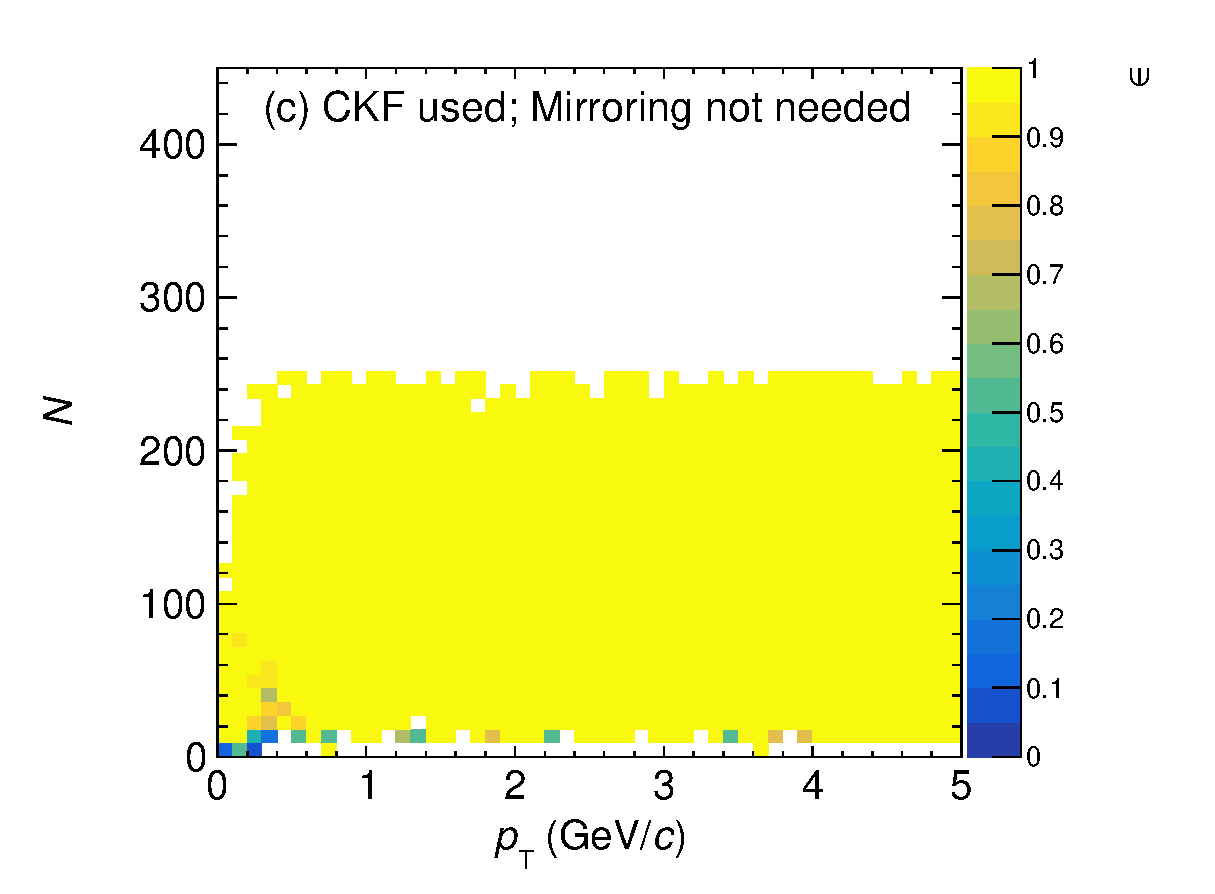
\includegraphics[width=\textwidth]{figures/Appendix/testNDGArMirrorEfficiencyVSNPointsVSpT_NoMirror.eps}
         \caption{}
         \label{fig:HP_Eff_CKF_NoMirror}
     \end{subfigure}
     \begin{subfigure}[b]{0.48\textwidth}
         \centering
         \includegraphics[width=\textwidth]{figures/Appendix/testNDGArMirrorEfficiencyVSNPointsVSpT_BKF_NoMirror.eps}
         \caption{}
         \label{fig:HP_Eff_BKF_NoMirror}
     \end{subfigure}
        \caption{\textcolor{red}{Xianguo Check: Reconstruction efficiency $\epsilon$ for the HP sample, as a function of the total number of points in the track $N$ and the initial true transverse momentum $p_\textrm{T}$. Analogous to Fig. \ref{fig:PS_Eff}}} \label{fig:HP_Eff}
\end{figure}
\clearpage

In Figs.~\ref{fig:ND-GArVSLArm} and~\ref{fig:ND-GArVSNPoints}, we show the relative momentum resolution and bias for the three particle types present in the HP sample, as a function of $L_\textrm{Arm}$ and $N$, respectively. These are analogous to Fig.~\ref{fig:ND-GArVSlength} in the main text.


\begin{figure}[!ht]
     \centering
     \begin{subfigure}[b]{0.43\textwidth}
         \centering
         \includegraphics[width=\textwidth]{figures/Appendix/RespVSLArm_XL.eps}
         \caption{}
         \label{fig:ResND-GArVSLArm}
     \end{subfigure}
     \begin{subfigure}[b]{0.43\textwidth}
         \centering
         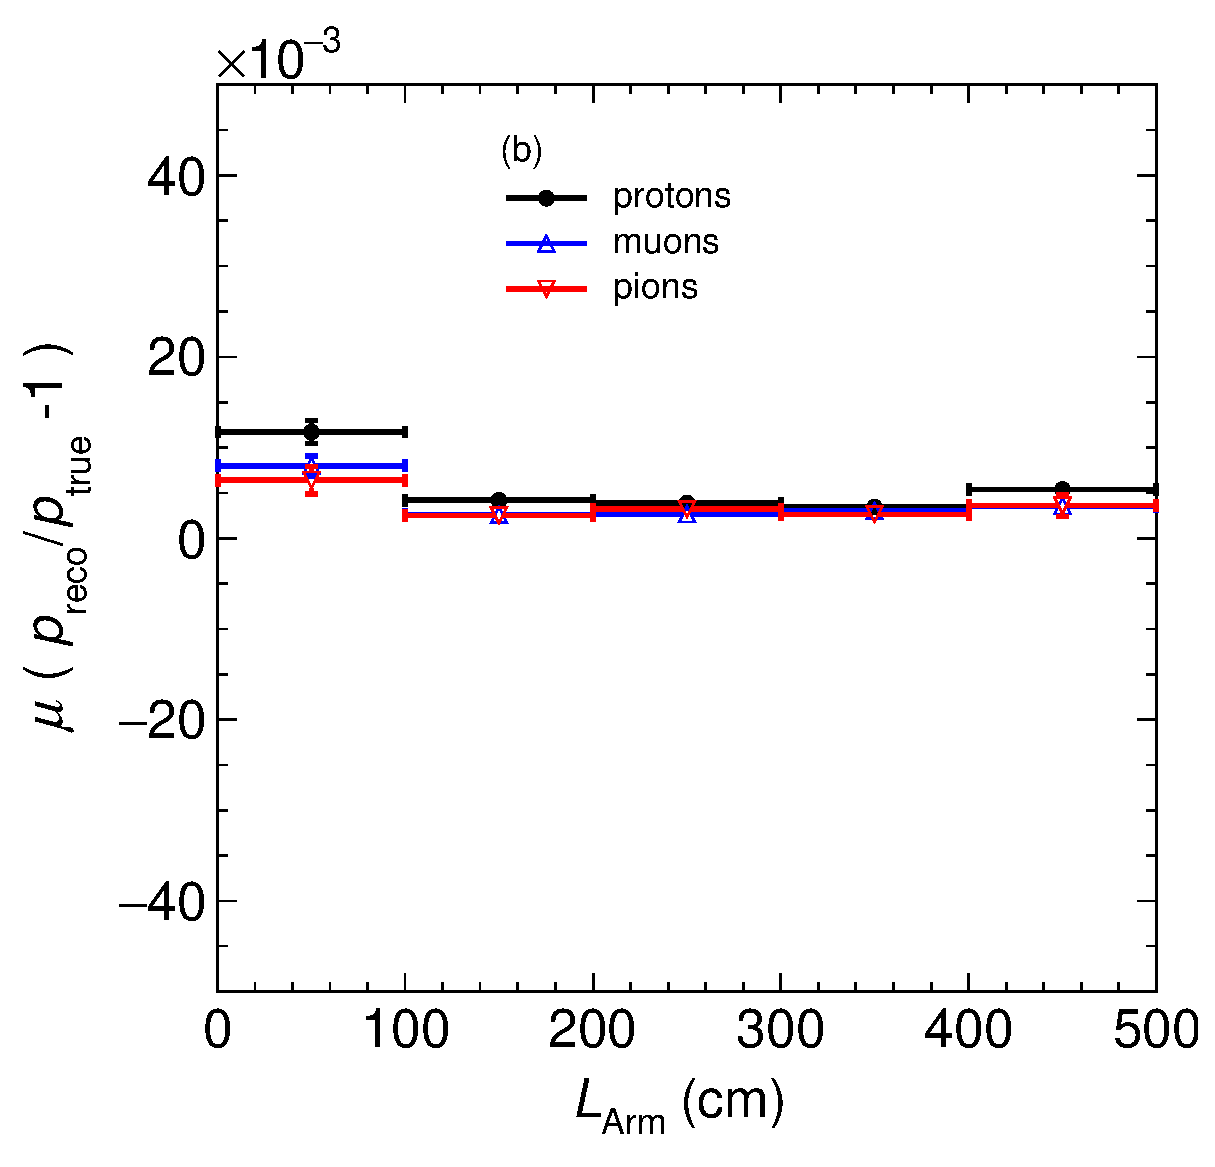
\includegraphics[width=\textwidth]{figures/Appendix/BiaspVSLArm_XL.eps}
         \caption{}
         \label{fig:BiasND-GArVSLArm}
     \end{subfigure}
        \caption{Similar plots to Fig.~\ref{fig:ND-GArVSp}. In this case the relative momentum resolution (a) and bias (b) are shown as a function of the tracks' lever arm $L_\textrm{Arm}$ for the HP sample. }
        \label{fig:ND-GArVSLArm}
\end{figure}

\begin{figure}[!ht]
     \centering
     \begin{subfigure}[b]{0.43\textwidth}
         \centering
         \includegraphics[width=\textwidth]{figures/Appendix/RespVSNPoints_XL.eps}
         \caption{}
         \label{fig:ResND-GArVSNPoints}
     \end{subfigure}
     \begin{subfigure}[b]{0.43\textwidth}
         \centering
         \includegraphics[width=\textwidth]{figures/Appendix/BiaspVSNPoints_XL.eps}
         \caption{}
         \label{fig:BiasND-GArVSNPoints}
     \end{subfigure}
        \caption{Similar plots to Fig.~\ref{fig:ND-GArVSp}. In this case the relative momentum resolution (a) and bias (b) are shown as a function of the number of points in the track $N$ for the HP sample.}
        \label{fig:ND-GArVSNPoints}
\end{figure}


